We evaluate whether analyzer evidence helps \toolname recover vulnerable-side warnings and reduce fixed-side reports.
The evaluation focuses on patch-local and patch-related-file behavior rather than whole-kernel bug discovery.

\subsection{Research Questions}

\noindent\textbf{RQ1: KNighter-derived checkers.} How does \toolname compare with KNighter's refinement loop on vulnerable-version warning coverage, fixed-side report burden and paired discrimination?

\noindent\textbf{RQ2: Cross-backend feasibility and cost.} Can the refinement layer operate on an archived CodeQL query associated with an earlier automatic generation run, and what integration and execution costs are observable?

\noindent\textbf{RQ3: Evidence contribution.} How do the native and no-internal variants differ, and what do their edits and reported gains establish?

\noindent\textbf{RQ4: Model sensitivity.} How does the workflow perform with three editor configurations on the same subset under common reply and output ceilings?

\subsection{Experimental Setup}

\subhead{Subjects and benchmarks.}
We organize the evaluation into four experiments (E1--E4).
E1 uses KNighter-derived Linux CSA checkers under patch-related object validation.
From 286 artifact records on 60 commits, 241 records on 39 commits lack an upstream refinement-status row.
We select one nonempty repaired-source artifact per commit by upstream TP, then TN, then the lowest checker index.
This fixed, non-random rule selects the inputs; independent paired replay supplies their starting outcomes.
All 39 enter KNighter refinement and both \toolname variants, including cases that remain noisy or fail to improve.
Initially, 15 checkers warn on both revisions and 24 are silent on both.
Their zero starting PDS is the study's entry state.

The 15 initially noisy checkers also form a complete report-refinement stratum.
Its results reuse the full-cohort outputs.
For the 24 silent starts, KNighter's no-report branch compiles without a model edit, whereas \toolname attempts recovery.
We report these branches as the systems execute them.

The selected implementation is v43, chosen after comparing two configurations on six experimental subjects.
Compatible executions on those subjects are reused in E1; the configuration-selection cases overlap the evaluation.
The artifact retains those trials and their reuse checks.
G04 uses its architecture-correct ARM64 scope and evidence after repair of an earlier wrong-object scan.

E2 uses an archived CodeQL input associated with an earlier automatic generation run, independently of KNighter, for ImageMagick (CVE-2017-12877, \texttt{coders/\allowbreak mat.c}).
All three refinement decodes start from this same query.
We report it separately from CSA.
Earlier 20-row results from mixed and manual inputs are excluded.
E3 compares native and no-internal on all 39 main pairs and repeats a 12-subject subset; E4 uses the same 12 subjects, native only, with three decodes per model (Figure~\ref{fig:study-design}).

Subset membership follows the initial scan status.
We sort SHA-256 hashes of a fixed artifact-recorded salt plus case ID within the original 14 noisy and 25 silent cases, then take the first 4 and 8.
A later scan repair corrects G08 from $0/0$ to $2/2$, leaving the same membership with 5 noisy and 7 silent subjects.
The selection uses no refinement outcomes or vulnerability-class stratification; it contains no bounds cases.

\begin{figure}[!htbp]
\centering
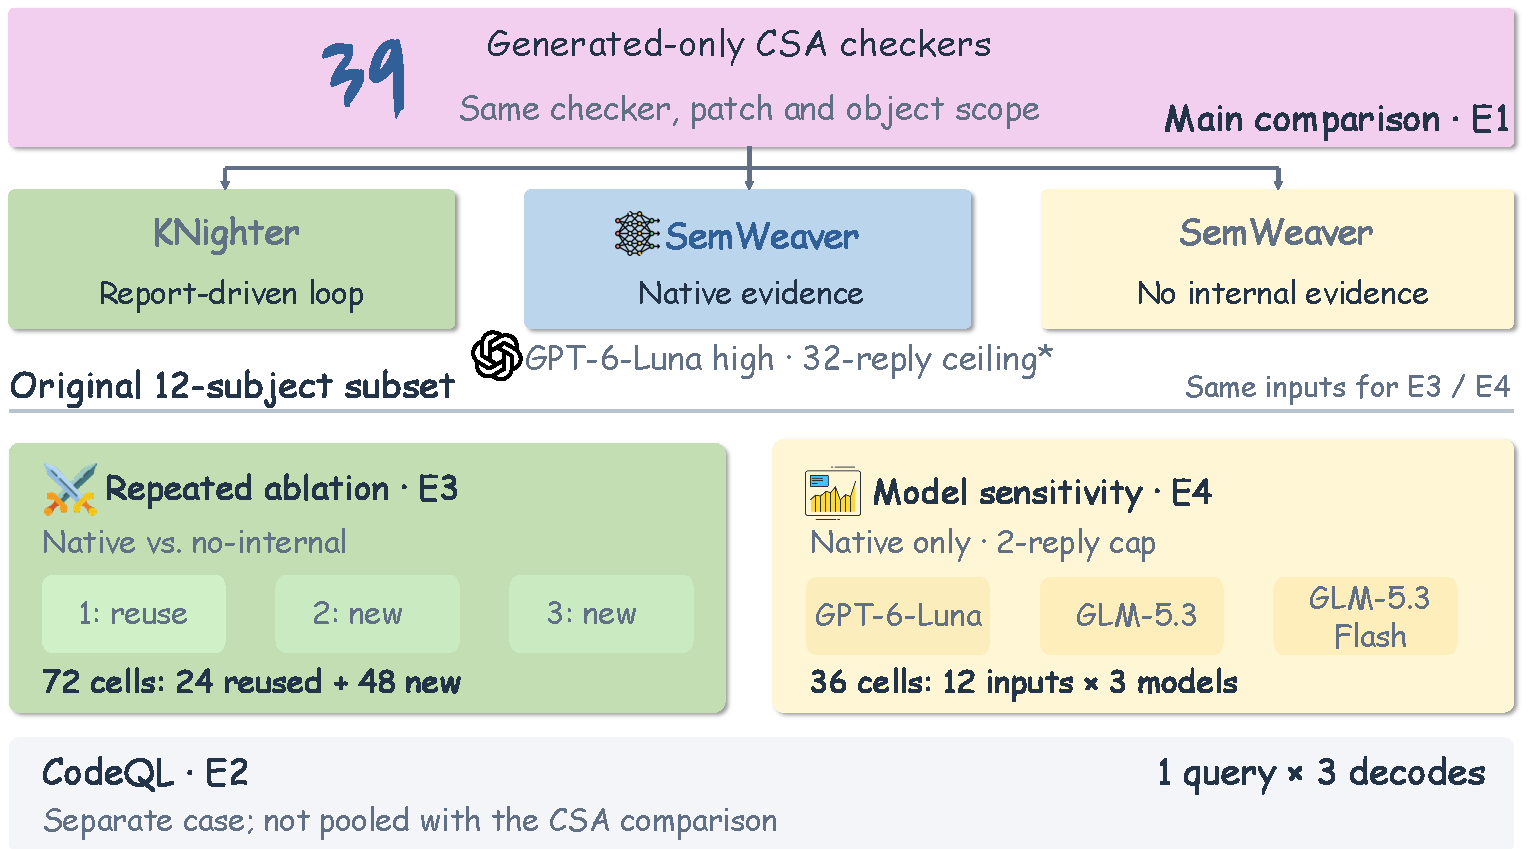
\includegraphics[width=0.70\textwidth]{figures/manual/study-design.pdf}
\Description{All 39 CSA checkers enter three main comparison arms. E3 and E4 use the same original 12-subject subset. E3 reuses 24 first-decode condition cells and adds 48. The drawing shows E4's first 36 native-only cells; two further decodes add 72, for 108 trial records. The CodeQL case is separate.}
\caption{\textbf{Experimental design and reuse.} E3's first decode reuses E1. The E4 panel depicts its first decode (36 cells); two further decodes add 72 cells, for 108 records on the same 12 inputs. Cells are not independent bugs. $^*$Audited natural-stop reuses retain original caps; shared ceilings do not imply equal realized effort.}
\label{fig:study-design}
\end{figure}

\subhead{Baselines and variants.}
We hold the generated detector fixed so that the comparison follows edits to the same checker rather than a fresh generation draw.
E1 native, no-internal and KNighter use the same requested GPT-6-Luna-high editor and a 32-reply ceiling.
KNighter retains its report-driven algorithm with five reports and two outer attempts, and its emitted checkers receive independent scans.
The 24 no-report branches consume no reply.
Two natural one-response No-FP stops are audited reuses that retain their original eight-reply ceiling; both terminate before either ceiling.
We report actual replies and warning counts alongside the common maximum.

Within \toolname, no-internal removes native compiler and checker-execution views while keeping the checker, patch, frozen source, build and paired-scan feedback, and stopping rule.
Native receives the bounded CFG witness and mismatch views and available dynamic observations.
E3 repeats the original 12 subjects at 32 replies and 16,384 output tokens per call.
E4 uses GPT-6-Luna high, GLM-5.3 high and GLM-5.3-Flash high, with three decodes per model, 2 replies per decode and 65,536 output tokens per call.
Actual GLM effort fields are retained.
Earlier default-effort, smaller-output and outside-subset histories are kept separate.
E4 has no no-internal arm across models.

\subhead{Experimental procedure.}
For each sample, we collect evidence, refine the detector and validate it on both revisions.
Each permitted reply counts as an attempt.
Compilable changed candidates receive independent paired replay and are retained under Equation~\ref{eq:accept}.
The next call receives the latest attempted code and feedback; the best retained detector is stored separately.
The loop stops when a vulnerable warning and fixed-side silence are achieved, after three valid validations without improvement, after three consecutive invalid model attempts, or at the reply cap.

We preserve failed attempts and consumed prefixes when repairing execution problems.
Thinking-only replies consume budget.
For one GLM reply containing an explicit action and three edits but no explanatory summary, network-disabled replay supplied an empty summary and reproduced the model-specified code with no new call.
Healthy zero-callback probes use static evidence.
Compilation failures, format failures, unavailable observations, provider interruptions and invalid scans remain distinct; no manual checker completion enters the scored results.

\subhead{Environment.}
CSA uses Clang/LLVM 18.1.3 and Python 3.12.3.
CodeQL uses version 2.26.4, \texttt{codeql/cpp-all} 8.0.3 and no-build databases.
Each Linux subject uses its patch commit and parent, \texttt{allyesconfig}, architecture-correct objects, and the same scope for starting, baseline and refined checkers.
Manifests record code, evidence and raw paired outputs.
The recorded model labels and high-effort requests identify the tested services.
Both Responses adapters omit the configured temperature field, and no fixed seed is used.

\subhead{Use of generative AI in the study.}
The editor models generated the checker and query edits evaluated in this study.
Codex assisted with the development of experimental tools.

\subsection{Metrics}

We report vulnerable-version warning presence and fixed-side report burden.
Let $n_v(D)$ and $n_f(D)$ count warnings in the same patch-related object scope on the vulnerable and fixed revisions.
The stronger outcome, \emph{patch-discriminating success} (PDS), requires a vulnerable-side warning and fixed-side silence:
\begin{equation}
\begin{aligned}
H_v(D,P,V)&=\mathbb{1}[\mathrm{alerts}(D,V_{\mathrm{vuln}},P)>0],\\
S_f(D,P,V)&=\mathbb{1}[\mathrm{alerts}(D,V_{\mathrm{fix}},P)=0],\\
\mathrm{PDS}(D,P,V)&=H_v(D,P,V)\land S_f(D,P,V).
\end{aligned}
\label{eq:pds}
\end{equation}
We distinguish two useful improvements.
\emph{Warning recovery} makes an initially silent vulnerable revision warning-positive, possibly with fixed-side noise.
\emph{Report reduction} lowers fixed-side reports while preserving vulnerable-side warning presence.
A detector that loses an existing vulnerable warning is rejected.
A comparative disadvantage means that another arm retains a better result, which may still be an improvement over the starting checker.

For retained detector $D^*$ and normally paired-executed candidate $C$, the improvement rule is:
\begin{equation}
\begin{aligned}
\mathrm{Accept}(C,D^*)={}&\mathrm{AnalyzerOK}(C)\land H_v(C)\\
&\land\bigl(\neg H_v(D^*)\lor n_f(C)<n_f(D^*)\bigr)\land Q(C).
\end{aligned}
\label{eq:accept}
\end{equation}
The editor requires a changed artifact before paired assessment.
$Q$ preserves required hits on controlled array fixtures in native and is identically true for no-internal.
This native-only guard records zero rejections in E1/E3.

For precision, recall and $F_1=2TP/(2TP+FP+FN)$, each vulnerable revision is a positive and its fixed revision a negative, classified by warning presence.
These metrics cover 78 patch-version decisions.
Fixed-side report counts measure inspection burden.
Neither measure adjudicates individual bug sites: G08, for example, warns on allocation failure rather than the registration-failure leak repaired by its patch.
The qualitative follow-up in Section~\ref{sec:target-results} examines target association separately; failed scans remain unscored.
